\documentclass[10pt]{book}
\author{Lan Peng, PhD Student\\ \\Department of Industrial and Systems Engineering\\University at Buffalo, SUNY\\lanpeng@buffalo.edu}
\title{Notes for Operations Research \& More}

\usepackage{amsmath, amssymb, amsthm}
\usepackage{color, soul}
\usepackage[left=1.5cm,right=1.5cm,top=1.5cm,bottom=1.5cm]{geometry}
\usepackage{tabularx}
\usepackage{tikz}
	\usetikzlibrary{shapes.geometric, arrows}
		\tikzstyle{roundedRectangle} = [rectangle, rounded corners, minimum width=3cm, minimum height=1cm,text centered, draw=black]
		\tikzstyle{io} = [trapezium, trapezium left angle=70, trapezium right angle=110, minimum width=3cm, minimum height=1cm, text centered, draw=black]
		\tikzstyle{process} = [rectangle, minimum width=2cm, minimum height=1cm, text centered, draw=black, inner sep=0.1cm]
		\tikzstyle{decision} = [diamond, minimum width=2cm, minimum height=0cm, text centered, draw=black, inner sep=0cm]
		\tikzstyle{arrow} = [thick,->,>=stealth]
		\tikzstyle{circleNode} = [circle, minimum size = 1cm, text centered, draw=black, inner sep=0.1cm]
\usepackage{algorithm}
\usepackage{algorithmic}
\usepackage{bm}
\usepackage{mathrsfs}
\usepackage{hyperref}
\usepackage{longtable}
\usepackage{makecell}
\usepackage{lscape}

\begin{document}
	\maketitle
	\tableofcontents

	\part{Preliminary Topics}
		\chapter{Review of Linear Algebra}

		\chapter{Convex Sets}

		\chapter{Convex Functions and Generalizations}

	\part{Linear Programming}
		\chapter{Formulation}
			\section{Typical Problems}

			\section{Formulation Skills}
				\subsection{Absolute Value}
					\framebox{\textbf{Description:}}
					Consider the following model statement:
					\begin{align}
						\min \quad & \sum_{j\in J}c_j|x_j|, \quad c_j > 0 \nonumber\\
						\text{s.t.} \quad & \sum_{j\in J}a_{ij}x_j \gtreqless b_i, \quad \forall i\in I \nonumber\\
						                  & x_j \quad \text{unrestricted}, \quad \forall j\in J \nonumber
					\end{align}
					\framebox{\textbf{Modeling:}}
					\begin{align}
						\min \quad & \sum_{j\in J}c_j(x_j^+ + x_j^-), \quad c_j > 0 \nonumber\\
						\text{s.t.} \quad & \sum_{j\in J}a_{ij}(x_j^+ - x_j^-) \gtreqless b_i, \quad \forall i\in I \nonumber\\
						                  & x_j^+, x_j^- \ge 0, \quad \forall j\in J \nonumber
					\end{align}

				\subsection{A Minimax Objective}
					\framebox{\textbf{Description:}}
					Consider the following model statement:
					\begin{align}
						\min \quad & \max_{k\in K}\sum_{j\in J}c_{kj}x_j \nonumber\\
						\text{s.t.} \quad & \sum_{j\in J}a_{ij}x_j \gtreqless b_i, \quad \forall i\in I \nonumber\\
						                  & x_j \ge 0, \quad \forall j\in J \nonumber
					\end{align}
					\framebox{\textbf{Modeling:}}
					\begin{align}
						\min \quad & z \nonumber\\
						\text{s.t.} \quad & \sum_{j\in J}a_{ij}x_j \gtreqless b_i, \quad \forall i\in I \nonumber\\
										  & \sum_{j\in J}c_{kj}x_j \le z, \quad \forall k\in K \nonumber\\
						                  & x_j \ge 0, \quad \forall j\in J \nonumber
					\end{align}
				\subsection{A fractional Objective}
					\framebox{\textbf{Description:}}
					Consider the following model statement:
					\begin{align}
						\min \quad & \frac{\sum_{j\in J}c_{j}x_j + \alpha}{\sum_{j\in J}d_{j}x_j + \beta} \nonumber\\
						\text{s.t.} \quad & \sum_{j\in J}a_{ij}x_j \gtreqless b_i, \quad \forall i\in I \nonumber\\
						                  & x_j \ge 0, \quad \forall j\in J \nonumber
					\end{align}
					\framebox{\textbf{Modeling:}}
					\begin{align}
						\min \quad & \sum_{j\in J}c_{j}x_jt + \alpha t \nonumber\\
						\text{s.t.} \quad & \sum_{j\in J}a_{ij}x_j \gtreqless b_i, \quad \forall i\in I \nonumber\\
										  & \sum_{j\in J}d_jx_jt + \beta t = 1\nonumber\\
										  & t > 0 \nonumber\\
						                  & x_j \ge 0, \quad \forall j\in J \nonumber\\
						                  & (t = \frac1{\sum_{j\in J}d_jx_j + \beta}) \nonumber
					\end{align}
				\subsection{A range Constraint}
					\framebox{\textbf{Description:}}
					Consider the following model statement:
					\begin{align}
						\min \quad & \sum_{j\in J}c_jx_j \nonumber\\
						\text{s.t.} \quad & d_i\le \sum_{j\in J}a_{ij}x_j \le e_i, \quad \forall i\in I \nonumber\\
						                  & x_j \ge 0, \quad \forall j\in J \nonumber
					\end{align}
					\framebox{\textbf{Modeling:}}
					\begin{align}
						\min \quad & \sum_{j\in J}c_jx_j, \quad c_j > 0 \nonumber\\
						\text{s.t.} \quad & u_i + \sum_{j\in J}a_{ij}x_j = e_i, \quad \forall i\in I \nonumber\\
						                  & x_j \ge 0, \quad \forall j\in J \nonumber\\
						                  & 0\le u_i \le e_i-d_i, \quad \forall i\in I \nonumber
					\end{align}

		\chapter{Simplex Method}
			\section{Basic Feasible Solutions and Extreme Points}

			\section{Simplex Method}

				\subsection{Simplex Method Algorithm}

				\subsection{Simplex Method Tableau}

				\subsection{Simplex Method as a Search Algorithm}

			\section{Revised Simplex Method}

			\section{Simplex Method with Bounded Variables}

			\section{Artificial Variable}
				\subsection{Two-Phase Method}

				\subsection{Big-M Method}

				\subsection{Single Artificial Variable Technique}

			\section{Degeneracy and Cycling}
				\subsection{Degeneracy}

				\subsection{Cycling}

				\subsection{Cycling Prevention Rules}
					\subsubsection{Lexicographic Rule}

					\subsubsection{Bland's Rule}

					\subsubsection{Successive Ratio Rule}

		\chapter{Duality Theory and Sensitivity Analysis}

		\chapter{Decomposition Principle}

		\chapter{Ellipsoid Algorithm}

		\chapter{Projective Algorithm}

		\chapter{Interior-Point Algorithm}

	\part{Graph and Network Theory}
		\chapter{Paths, Trees, and Cycles}

		\chapter{Shortest-Path Problem}

		\chapter{Minimum Spanning Tree Problem}

		\chapter{Maximum Flow Problem}

		\chapter{Minimum Cost Flow Problem}

		\chapter{Assignment and Matching Problem}

		\chapter{Graph Algorithms}
		
		\chapter{Polygon Triangulation}
			\section{Types of Polygons}
				\framebox{\textbf{Def:}} A \textbf{simple polygon} is a closed polygonal curve without self-intersection.
				\begin{figure}[h!]
					\centering
					\begin{tikzpicture}
						\draw (0, 0) -- (3, -1) -- (4, 3) -- (2, 4) -- (0, 0);
						\draw (6, 3) -- (8, -1) -- (9, 2) -- (5.5, 0) -- (6, 3);
						\node at (2, -1.5) [below] {Simple Polygon};
						\node at (7.5, -1.5) [below] {Non-simple Polygon};
					\end{tikzpicture}
				\end{figure}
				Polygons are basic building blocks in most geometric applications. It can model arbitrarily complex shapes, and apply simple algorithms and algebraic representation/manipulation.
			\section{Triangulation}
				\framebox{\textbf{Def:}} \textbf{Triangulation} is to partition polygon $P$ into non-overlapping triangles using diagonals only. It reduces complex shapes to collection of simpler shapes. Every simple $n$-gon admits a triangulation which has $n-2$ triangles.
				
			\section{Art Gallery Theorem}
				\framebox{\textbf{Scenario}}: The floor plan of an art gallery modeled as a simple polygon with $n$ vertices, there are guards which is stationed at fixed positions with 360 degree vision but cannot see through the walls. How many guards does the art gallery need for the security? (Fun fact: This problem was posted to Vasek Chvatal by Victor Klee in 1973)				

	\part{Integer and Combinatorial Programming}
		\chapter{Formulation}
			\section{Typical Problems}

			\section{Integer Programming Formulation Skills}
				\subsection{A Variable Taking Discontinuous Values}
					\framebox{\textbf{Description:}} In algebraic notation: 
					\begin{equation}
						x = 0,\quad \text{or} \quad l\le x \le u \nonumber
					\end{equation}
					\framebox{\textbf{Modeling:}}
					\begin{align}
						& x \le uy\nonumber \\
						& x \ge ly \nonumber \\
						& y \in \{0, 1\} \nonumber
					\end{align}
					where
					\begin{equation}y=\begin{cases}0, & \text{if }x=0 \\ 1, & \text{if } l\le x \le u\end{cases}\nonumber \end{equation}
						
				\subsection{Fixed Costs}
					\framebox{\textbf{Description:}} In algebraic notation: 
					\begin{equation}
						C(x) = \begin{cases} 0 & \text{for } x=0 \\ k + cx & \text{for } x > 0 \end{cases} \nonumber
					\end{equation}
					\framebox{\textbf{Modeling:}}
					\begin{align}
						& C^*(x, y) = ky+cx\nonumber\\
						& x \le My \nonumber \\
						& x \ge 0 \nonumber\\
						& y \in \{0, 1\} \nonumber
					\end{align}
					where
					\begin{equation}y=\begin{cases}0, & \text{if }x=0 \\ 1, & \text{if }x\ge 0\end{cases}\nonumber \end{equation}
				
				\subsection{Either-or Constraints}
					\framebox{\textbf{Description:}} In algebraic notation: 
					\begin{equation}
						\sum_{j\in J} a_{1j} x_j \le b_1 \text{ or } \sum_{j\in J} a_{2j} x_j \le b_2 \nonumber
					\end{equation}
					\framebox{\textbf{Modeling:}}
					\begin{align}
						& \sum_{j\in J} a_{1j} x_j \le b_1 + M_1y \nonumber \\
						& \sum_{j\in J} a_{2j} x_j \le b_2 + M_1(1-y) \nonumber \\
						& y \in \{0, 1\} \nonumber
					\end{align}
					where
					\begin{equation}y=\begin{cases}0, & \text{if }\sum_{j\in J} a_{1j} x_j \le b_1 \\ 1, & \text{if } \sum_{j\in J} a_{2j} x_j \le b_2\end{cases}\nonumber \end{equation}
					Notice that the sign before $M$ is determined by the inequality $\ge$ or $\le$, if it is \lq\lq{}$\ge$\rq\rq{}, use \lq\lq{}$-$\rq\rq{}, if it \lq\lq{}$\le$\rq\rq{}, use \lq\lq{}+\rq\rq{}.
				
				\subsection{Conditional Constraints}
					\framebox{\textbf{Description:}} If constraint A is satisfied, then constraint B must also be satisfied
					\begin{equation}
						\text{If} \quad \sum_{j\in J} a_{1j} x_j \le b_1 \text{ then } \sum_{j\in J} a_{2j} x_j \le b_2 \nonumber
					\end{equation}
					The key part is to find the opposite of the first condition. We are using $A\Rightarrow B \Leftrightarrow \neg B \Rightarrow \neg A$\\
					Therefore it is equivalent to
					\begin{equation}
						\sum_{j\in J} a_{1j} x_j > b_1 \text{ or } \sum_{j\in J} a_{2j} x_j \le b_2 \nonumber
					\end{equation}
					Furthermore, it is equivalent to
					\begin{equation}
						\sum_{j\in J} a_{1j} x_j \ge b_1 + \epsilon \text{ or } \sum_{j\in J} a_{2j} x_j \le b_2 \nonumber
					\end{equation}
					Where $\epsilon$ is a very small positive number.\\
					\framebox{\textbf{Modeling:}}
					\begin{align}
						& \sum_{j\in J} a_{1j} x_j \ge b_1 + \epsilon -  M_2y \nonumber \\
						& \sum_{j\in J} a_{2j} x_j \le b_2 + M_2(1-y) \nonumber \\
						& y \in \{0, 1\} \nonumber
					\end{align}	
				
				\subsection{Special Ordered Sets}
					\framebox{\textbf{SOS1 Description}} Out of a set of yes-no decisions, at most one decision variable can be yes. \
					\begin{align}
						x_1=1,x_2=x_3&=\dots=x_n=0 \nonumber \\
						&\text{or} \nonumber \\
						x_2=1, x_1=x_3&=\dots=x_n=0 \nonumber \\
						&\text{or ...} \nonumber
					\end{align} 
					\framebox{\textbf{Modeling:}}
					\begin{equation} \sum_{i} x_i = 1, \quad i \in N\nonumber \end{equation}
					\framebox{\textbf{SOS2 Description 1}} Out of a set of binary variables, at most two variables can be nonzero. In addition, the two variables must be adjacent to each other in a fixed order list.\\
					\framebox{\textbf{Modeling:}}
					If $x_1, x_2, ... , x_n$ is a SOS2, then
					\begin{align}
						& \sum_{i=1}^{n} x_i \le 2 \nonumber \\
						& x_i + x_j \le 1, \forall i \in \{1, 2,..., n\}, j \in \{i+2, i+3, ..., n\} \nonumber \\
						&x_i \in \{0, 1\}\nonumber
					\end{align}
					\framebox{\textbf{SOS2 Description 2}} There is another type of definition, that is out of a set of nonnegative variables \textbf{not binary here}, at most two variables can be nonzero. In addition, the two variables must be adjacent to each other in a fixed order list. All variables summing to 1.\\
					This definition of SOS2 is used in the following section \textit{Piecewise Linear Formulations}\\
									
				\subsection{Piecewise Linear Formulations}
					\framebox{\textbf{Description:}} The objective function is a sequence of line segments, e.g. $y=f(x), $ consists $k-1$ linear segments going through $k$ given points $(x_1, y_1), (x_2, y_2), ... ,(x_k, y_k)$.\\
					Denote 
					\begin{equation}d_i=\begin{cases}1, & x\in (x_i, x_{i+1})\\0, & \text{otherwise} \end{cases}\nonumber\end{equation}
					Then the objective function is
					\begin{equation}\sum_{i \in \{1, 2, ..., k-1\}} y = d_if_i(x)\nonumber \end{equation} 
					\framebox{\textbf{Modeling:}} Given that objective function as a piecewise linear formulation, we can have these constraints\\
					\begin{align}
						&\sum_{i \in \{1, 2, ..., k-1\}} d_i =1 \nonumber \\
						&d_i \in \{0, 1\}, i \in \{1, 2, ..., k-1\} \nonumber \\
						& x = \sum_{i \in \{1, 2, ..., k\}} w_i x_i \nonumber \\
						& y = \sum_{i \in \{1, 2, ..., k\}} w_i y_i \nonumber \\
						& w_1 \le d_1 \nonumber \\
						& w_i \le d_{i-1} + d{i}, i \in \{2, 3, ..., k-1\} \nonumber \\
						& w_k \le d_{k-1} \nonumber
					\end{align}
					In this case, $ w_i \in SOS2$ (second definition)		
										
				\subsection{Conditional Binary Variables}
					\framebox{\textbf{Description:}} Choose at most $n$ binary variable to be 1 out of  $x_1, x_2, ... x_m, m\ge n$. If $n=1$ then it is SOS1.\\
					\framebox{\textbf{Modeling:}}
					\begin{equation}
						\sum_{k\in \{1,2,...,m\}} x_k \le n\nonumber
					\end{equation}
					\framebox{\textbf{Description:}} Choose exactly $n$ binary variable to be 1 out of  $x_1, x_2, ... x_m, m\ge n$\\
					\framebox{\textbf{Modeling:}}
					\begin{equation}
						\sum_{k\in \{1,2,...,m\}} x_k = n\nonumber
					\end{equation}
					\framebox{\textbf{Description:}} Choose $x_j$ only if $x_k = 1$\\
					\framebox{\textbf{Modeling:}}
					\begin{equation}x_j = x_k \nonumber \end{equation}
					\framebox{\textbf{Description:}} \lq\lq{}and\rq\rq{} condition, iff $x_1, x_2, ... , x_m =1$ then $y=1$\\
					\framebox{\textbf{Modeling:}}
					\begin{align}
						& y \le x_i, i\in \{1, 2, ..., m\} \nonumber \\
						& y \ge \sum_{i \in \{1, 2, ..., m\}} x_i - (m - 1) \nonumber
					\end{align}

				\subsection{Elimination of Products of Variables}
					\framebox{\textbf{Description:}} For variables $x_1$ and $x_2$,
					\begin{equation}y = x_1 x_2\nonumber\end{equation}
					\framebox{\textbf{Modeling:}} If $x_1, x_2$ are binary, it is the same as \lq\lq{}and\rq\rq{} condition of binary variables.\\
					If $x_1$ is binary, while $x_2$ is continuous and $0 \le x_2 \le u$, then
					\begin{align}
						y &\le ux_1 \nonumber \\
						y &\le x_2 \nonumber \\
						y &\ge x_2 - u(1- x_1) \nonumber \\
						y &\ge 0 \nonumber
					\end{align}
					If both $x_1$ and $x_2$ are continuous, it is non-linear, we can use Piecewise linear formulation to simulate.

		\chapter{Branch and Bound}

		\chapter{Branch and Cut}

		\chapter{Packing and Matching}

		\chapter{Traveling Salesman Problem}

		\chapter{Knapsack Problem}

	\part{Nonlinear Programming}
		\chapter{KKT Optimality Conditions}

		\chapter{Lagrangian Duality}

		\chapter{Unconstrained Optimization}

		\chapter{Penalty and Barrier Functions}

	\part{Algorithms and Computational Complexity}
		\chapter{Computational Complexity}

		\chapter{Sorting}
			\section{Elementary Sorting Algorithms}

			\section{Heap-sort}

			\section{Quick-sort}

			\section{Sorting in Linear Time}

			\section{Medians and Order Statistics}

		\chapter{Data Structures}
			\section{Elementary Data Structures}

			\section{Hash Tables}

			\section{Binary Search Trees}

			\section{Red-Black Trees}

			\section{B-Trees}

			\section{Fibonacci Heaps}

			\section{van Emde Boas Trees}

		\chapter{Design and Analysis Techniques}
			\section{Dynamic Programming}

			\section{Greedy Algorithms}

			\section{Amortized Analysis}

			\section{Multi-threaded Algorithms}

			\section{Matrix Operations}

			\section{Polynomials and the FFT}

			\section{Number-Theoretic Algorithms}

			\section{String Matching}

			\section{Computational Geometry}

			\section{NP-Completeness}

			\section{Approximation Algorithms}

	\part{Heuristics ans Meta-heuristics}

	\part{Game Theory}
		\chapter{Games with Ordinal Payoffs}
			\section{Ordinal Games in Strategic Form}

			\section{Perfect-information Games}

			\section{General Dynamic Games}

		\chapter{Games with Cardinal Payoffs}
			\section{Expected Utility Theory}

			\section{Strategic-form Games}

			\section{Extensive-form Games}

		\chapter{Knowledge, Common Knowledge, Beliefs}
			\section{Common Knowledge}

			\section{Adding Beliefs to Knowledge}

			\section{Rationality}

		\chapter{Refinements of Subgame-perfect Equilibrium}
			\section{Weak Sequential Equilibrium}

			\section{Sequential Equilibrium}

			\section{Perfect Bayesian Equilibrium}

		\chapter{Incomplete Information}
			\section{Static Games}

			\section{Dynamic Games}

			\section{The Type-Space Approach}

	\part{Decision Analysis}
	

	\part{Probability, Stochastic Processes and Markov Chains}
		\chapter{Probability}

		\chapter{Random Variables}
			\section{Relationship between Some Random Variables}
				\begin{figure}[h]
					\centering
					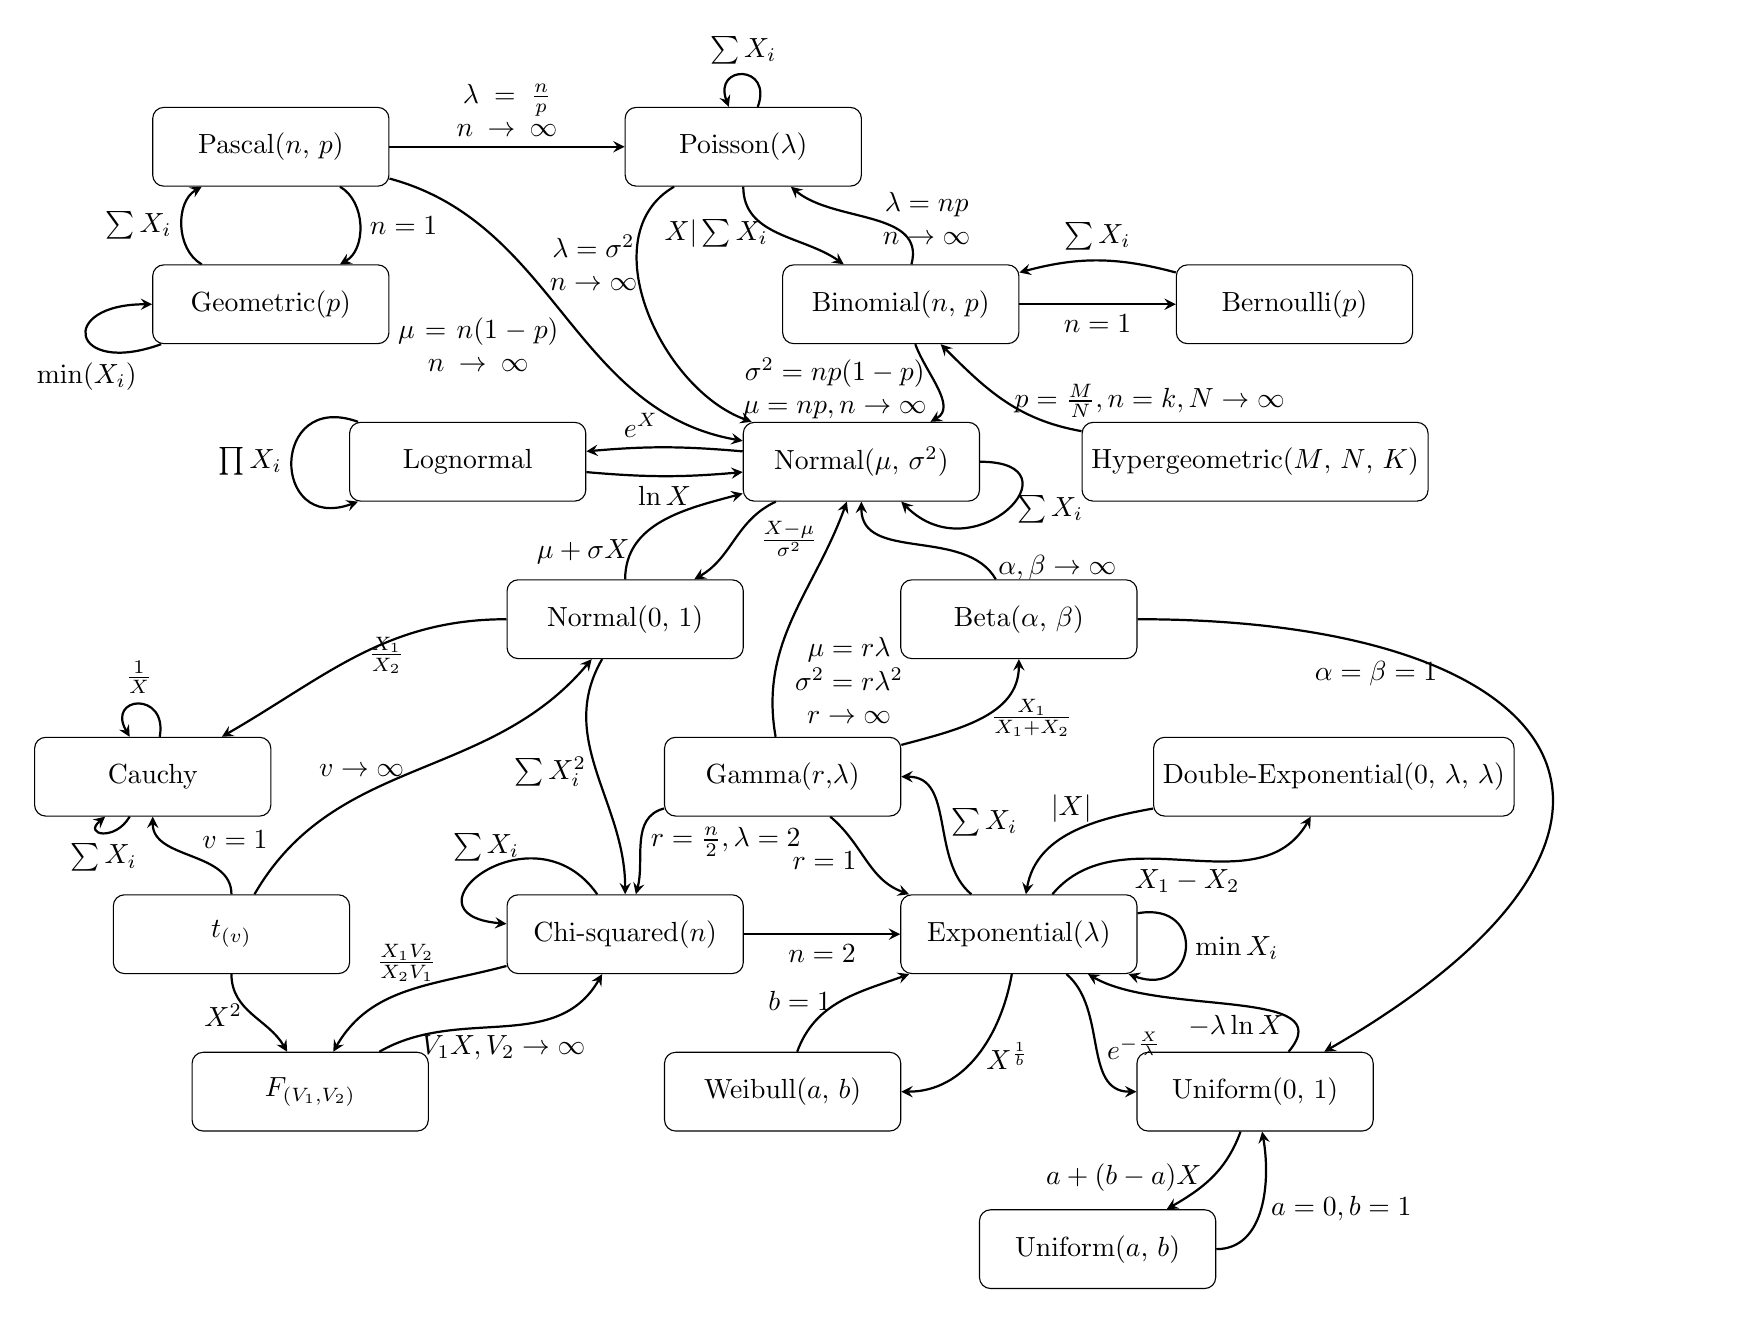
\begin{tikzpicture}[node distance = 2cm]
						\node (Pascal) [roundedRectangle] {Pascal($n$, $p$)};
						\node (Poisson) [roundedRectangle, xshift = 6cm] {Poisson($\lambda$)};
						\node (Geometric) [roundedRectangle, below of = Pascal] {Geometric($p$)};
						\node (Binomial) [roundedRectangle, below of = Poisson, xshift = 2cm] {Binomial($n$, $p$)};
						\node (Bernoulli) [roundedRectangle, below of = Poisson, xshift = 7cm] {Bernoulli($p$)};
						\node (Lognormal) [roundedRectangle, below of = Geometric, xshift = 2.5cm] {Lognormal};
						\node (Normal) [roundedRectangle, below of = Geometric, xshift = 7.5cm] {Normal($\mu$, $\sigma^2$)};
						\node (Hypergeometric) [roundedRectangle, below of = Geometric, xshift = 12.5cm] {Hypergeometric($M$, $N$, $K$)};
						\node (SNormal) [roundedRectangle, below of = Lognormal, xshift=2cm] {Normal(0, 1)};
						\node (Beta) [roundedRectangle, below of = Lognormal, xshift = 7cm] {Beta($\alpha$, $\beta$)};
						\node (DExponential) [roundedRectangle, below of = Beta, xshift = 4cm] {Double-Exponential($0$, $\lambda$, $\lambda$)};
						\node (Cauchy) [roundedRectangle, below of = SNormal, xshift = -6cm] {Cauchy};
						\node (Gamma) [roundedRectangle, below of = SNormal, xshift = 2cm] {Gamma($r$,$\lambda$)};
						\node (tv) [roundedRectangle, below of = Cauchy, xshift = 1cm] {$t_{(v)}$};
						\node (Chi-squared) [roundedRectangle, below of = Gamma, xshift = -2cm] {Chi-squared($n$)};
						\node (Exponential) [roundedRectangle, below of = Gamma, xshift = 3cm] {Exponential($\lambda$)};
						\node (Fvv) [roundedRectangle, below of = tv, xshift = 1cm] {$F_{(V_{1},V_{2})}$};
						\node (Weibull) [roundedRectangle, below of = Exponential, xshift = -3cm] {Weibull($a$, $b$)};
						\node (SUniform) [roundedRectangle, below of = Exponential, xshift = 3cm] {Uniform($0$, $1$)};
						\node (Uniform) [roundedRectangle, below of = SUniform, xshift = -2cm] {Uniform($a$, $b$)};
						\draw [arrow] (Pascal) to [out = -30, in = 30] node [right] {$n=1$} (Geometric);
						\draw [arrow] (Pascal) -- node [above, align=center, text width=2.5cm] {$\lambda=\frac{n}{p}$ \\ $n\rightarrow \infty$} (Poisson);
						\draw [arrow] (Pascal) to [out = -15, in = 170] node [below, align=center, text width=2.5cm, yshift=0.1cm, xshift=-1.1cm] {$\mu = n(1-p)$ \\ $n\rightarrow \infty$} (Normal);
						\draw [arrow] (Geometric) to [out = 150, in = -150] node [left] {$\sum X_i$} (Pascal);
						\draw [arrow] (Geometric) to [out = -160, in = 180, looseness=6] node [below, yshift = -0.2cm] {$\min(X_i)$} (Geometric);
						\draw [arrow] (Poisson) to [out = 70, in = 110, looseness=4] node [above] {$\sum X_i$} (Poisson);
						\draw [arrow] (Poisson) to [out = -90, in = 145] node [left] {$X|\sum X_i$} (Binomial);
						\draw [arrow] (Poisson) to [out = -150,in = 160] node [left, align=center, yshift=0.6cm] {$\lambda=\sigma^2$ \\ $n\rightarrow \infty$} (Normal);
						\draw [arrow] (Binomial) to [out = 75, in = -40] node [right, align=center] {$\lambda=np$ \\ $n\rightarrow \infty$} (Poisson);
						\draw [arrow] (Binomial) -- node [below] {$n=1$} (Bernoulli);
						\draw [arrow] (Bernoulli) to [out = 165, in = 15] node [above] {$\sum X_i$} (Binomial);
						\draw [arrow] (Binomial) to [out = -70, in = 30, align=center] node [left] {$\sigma^2=np(1-p)$ \\ $\mu=np, n\rightarrow \infty$} (Normal);
						\draw [arrow] (Hypergeometric) to [out = 170, in = -45] node [right] {$p=\frac{M}{N}, n=k, N\rightarrow \infty$} (Binomial);
						\draw [arrow] (Normal) to [out = 0, in = -45, looseness=3] node [right] {$\sum X_i$} (Normal);
						\draw [arrow] (Normal) to [out = 175, in = 5] node [above, xshift=-0.3cm] {$e^{X}$} (Lognormal);
						\draw [arrow] (Normal) to [out = -155, in = 30] node [right, xshift=0.2cm] {$\frac{X-\mu}{\sigma^2}$} (SNormal); 
						\draw [arrow] (Lognormal) to [out = -5, in = -175] node [below] {$\ln X$} (Normal);
						\draw [arrow] (Lognormal) to [out = 160, in = -160, looseness = 3] node [left] {$\prod X_i$} (Lognormal);
						\draw [arrow] (SNormal) to [out = 90, in = -165] node [left, yshift = -0.4cm, xshift = -0.3cm] {$\mu + \sigma X$} (Normal);
						\draw [arrow] (Beta) to [out = 120, in = -90] node [right, yshift=-0.3cm, xshift=0.9cm] {$\alpha, \beta \rightarrow \infty$} (Normal);
						\draw [arrow] (Beta) to [out = 0, in = 30, looseness=2.4] node [right, yshift=1cm, xshift=-3cm] {$\alpha=\beta=1$} (SUniform);
						\draw [arrow] (Gamma) to [out = 100, in = -110] node [right, align = center, yshift=-0.8cm, xshift = -0.1cm] {$\mu=r\lambda$\\$\sigma^2=r\lambda^2$\\$r\rightarrow \infty$} (Normal); 
						\draw [arrow] (Gamma) to [out = 15, in = -90] node [right] {$\frac{X_1}{X_1 + X_2}$} (Beta);
						\draw [arrow] (Gamma) to [out = -165, in = 75] node [right] {$r=\frac{n}{2}, \lambda=2$} (Chi-squared);
						\draw [arrow] (Gamma) to [out = -40, in = 160] node [left] {$r=1$} (Exponential);
						\draw [arrow] (SNormal) to [out = 180, in = 30] node [right] {$\frac{X_1}{X_2}$} (Cauchy);
						\draw [arrow] (SNormal) to [out = -120, in =90] node [left] {$\sum X_i^2$} (Chi-squared);
						\draw [arrow] (Cauchy) to [out = 80, in = 120, looseness = 4] node [above] {$\frac{1}{X}$} (Cauchy);
						\draw [arrow] (Cauchy) to [out = -120, in = -140, looseness = 3] node [below] {$\sum X_i$} (Cauchy);
						\draw [arrow] (tv) to [out = 90, in = -90] node [right, yshift = 0.2cm] {$v=1$} (Cauchy);
						\draw [arrow] (tv) to [out = 60, in = -130] node [left] {$v\rightarrow \infty$} (SNormal);
						\draw [arrow] (tv) to [out = -90, in = 120] node [left] {$X^2$} (Fvv);
						\draw [arrow] (Fvv) to [out = 30, in = -120] node [below] {$V_1X, V_2\rightarrow \infty$} (Chi-squared);
						\draw [arrow] (Chi-squared) to [out = -165, in = 60] node [above] {$\frac{X_1V_2}{X_2V_1}$} (Fvv);
						\draw [arrow] (Chi-squared) to [out = 125, in = 175, looseness = 3] node [above] {$\sum X_i$} (Chi-squared);
						\draw [arrow] (Chi-squared) -- node [below] {$n=2$} (Exponential);
						\draw [arrow] (Exponential) to [out = 140, in = 0] node [right] {$\sum X_i$} (Gamma);
						\draw [arrow] (Exponential) to [out = 50, in = -120] node [below] {$X_1 - X_2$} (DExponential);
						\draw [arrow] (Exponential) to [out = 10, in = -20, looseness = 3] node [right] {$\min X_i$} (Exponential);
						\draw [arrow] (Exponential) to [out = -40, in = 180] node [right] {$e^{-\frac{X}{\lambda}}$} (SUniform);
						\draw [arrow] (Exponential) to [out = -100, in = 0] node[right] {$X^{\frac{1}{b}}$} (Weibull);
						\draw [arrow] (DExponential) to [out = -170, in = 80] node [above] {$|X|$} (Exponential);
						\draw [arrow] (Uniform) to [out = 0, in = -80] node [right] {$a=0, b=1$} (SUniform);
						\draw [arrow] (SUniform) to [out = 50, in = -30] node [below] {$-\lambda \ln X$} (Exponential);
						\draw [arrow] (SUniform) to [out = -110, in = 30] node [left] {$a+(b-a)X$} (Uniform);
						\draw [arrow] (Weibull) to [out = 70, in = -160] node [left] {$b=1$} (Exponential);
					\end{tikzpicture}
					\caption{Relationship between Some Random Variables}
				\end{figure}

			\begin{landscape}
			\section{Discrete Random Variables}
				\begin{longtable}[c]{|c|c|c|c|c|c|}
					\caption{Discrete Random Variables \label{DRV}}\\
					\hline
					Distribution & PMF & CDF & Expectation & Variance & MGF \\
					\hline
					\endfirsthead
					\hline
					Distribution & PMF & CDF & Expectation & Variance & MGF \\
					\hline
					\endhead
					Discrete Uniform$(a, b)$ & 
					\makecell{$f(x)=\frac1{b-a+1}$ \\ $x=a, a+1, ..., b$} & 
					\makecell{$F(x)=\frac{x-a+1}{b-a+1}$ \\ $x=a, a+1, ..., b$} & 
					$E[X]=\frac{b-a}{2}$ & 
					$D[X]=\frac{(b-a+1)^2-1}{12}$ & 
					\makecell{$M(t)=\frac{e^{at}-e^{(b+1)t}}{(b-a+1)(1-e^t)}$ \\ $t \in \mathbb{R}$} \\
					\hline
					Bernoulli$(p)$ & 
					\makecell{$f(x)=p^x(1-p)^{1-x}$ \\ $x \in \{0,1\}$} &
					$F(x)=\begin{cases}0, \quad x<0 \\ 
										1-p, \quad 0\le x \le 1 \\
										1, \quad x>1\end{cases}$ & 
					$E[X]=p$ & 
					$D[X]=p(1-p)$ & 
					\makecell{$M(t)=1-p+pe^{t}$ \\ $t\in \mathbb{R}$}\\
					\hline
					Binomial$(n, p)$ &
					\makecell{$f(x)=\left(\begin{matrix}n\\x\end{matrix}\right)p^x(1-p)^{n-x}$ \\ $x=0,1,...,n$} &
					\makecell{$F(x)=\sum_{k=0}^{x}\left(\begin{matrix}n\\k\end{matrix}\right)p^k(1-p)^{n-k}$ \\ $x=0,1,...,n$} &
					$E[X]=np$ &
					$D[X]=np(1-p)$ &
					\makecell{$M(t)=(1-p+pe^{t})^n$ \\ $t\in \mathbb{R}$}\\
					\hline
					Poisson$(\mu)$ &
					\makecell{$f(x)=\frac{\mu^xe^\mu}{x!}$ \\ $x = 0,1,...,n,...$} &
					\makecell{$f(x)=\frac{\Gamma(x+1, \mu)}{\Gamma(x+1)}$ \\ $x=0,1,...,n,...$} &
					$E[X]=\mu$ &
					$D[X]=\mu$ &
					\makecell{$M(t)=e^{\mu(e^t-1)}$ \\ $t\in \mathbb{R}$} \\
					\hline
					Geometric$(p)$ &
					\makecell{$f(x)=p(1-p)^x$ \\ $x=0,1,...,n,...$} &
					\makecell{$F(x)=1-(1-p)^{x+1}$ \\ $x=0,1,...,n,...$} &
					$E[X]=\frac{1-p}p$ &
					$D[X]=\frac{1-p}{p^2}$ &
					\makecell{$M(t)=\frac{p}{1-(1-p)e^t}$ \\ $t < -\ln(1-p)$}\\
					\hline
					Pascal$(n, p)$ &
					\makecell{$f(x)=\left(\begin{matrix}n-1+x\\x\end{matrix}\right)p^n(1-p)^x$ \\ $x=0,1,2,...,n,...$} &
					\makecell{$F(x)=1-I_p(k+1,n)$ \\ $x=0,1,2,...,n,...$} &
					$E[X]=\frac{n(1-p)}{p}$&
					$D[X]=\frac{n(1-p)}{p^2}$ &
					\makecell{$M(t)=(\frac{p}{1-(1-p)e^t})^n$ \\ $t < -\ln(1-p)$}\\
					\hline
				\end{longtable}

			\section{Continuous Random Variables}
				\begin{longtable}[c]{|c|c|c|c|c|c|}
					\caption{Continuous Random Variables \label{CRV}}\\
					\hline
					Distribution & PDF & CDF & Expectation & Variance & MGF \\
					\hline
					\endfirsthead
					\hline
					Distribution & PDF & CDF & Expectation & Variance & MGF \\
					\hline
					\endhead
					Uniform$(a, b)$ & 
					\makecell{$f(x)=\frac1{b-a}$ \\ $x=[a,b]$} & 
					\makecell{$F(x)=\frac{x-a}{b-a}$ \\ $x=[a,b]$} & 
					$E[X]=\frac{b-a}{2}$ & 
					$D[X]=\frac{(b-a)^2}{12}$ & 
					$M(t)=\begin{cases}1, \quad t=0 \\ \frac{e^{bt}-e^{at}}{t(b-a)}, \quad t\ne 0\end{cases}$\\
					\hline
					Normal$(\mu, \sigma)$ &
					\makecell{$f(x)=\frac{1}{\sqrt{2\pi}\sigma}e^{-\frac{(x-\mu)^2}{2\sigma^2}}$ \\ $x\in \mathbb{R}$} &
					\makecell{$F(x)=\int_{-\infty}^{x}\frac{1}{\sqrt{2\pi}\sigma}e^{-\frac{(x-\mu)^2}{2\sigma^2}}$ \\ $x\in \mathbb{R}$} &
					$E[X]=\mu$ &
					$D[X]=\sigma^2$ &
					\makecell{$e^{\frac{t(t\sigma^2+2\mu)}{2}}$ \\ $t\in \mathbb{R}$}\\
					\hline
					Exponential$\lambda)$ &
					\makecell{$f(x)=\lambda e^{-\lambda x}$ \\ $x>0$} &
					\makecell{$F(x)=1-e^{\lambda x}$ \\ $x>0$} &
					$E[X]=\frac{1}{\lambda}$ &
					$D[X]=\frac{1}{\lambda^2}$ &
					\makecell{$\frac{1}{1-\frac{t}{\lambda}}$ \\ $t<\lambda$}\\
					\hline
					Erlang$(n, \lambda)$ &
					\makecell{$f(x)=\frac{\lambda^n x^{n-1} e^{-\lambda x}}{(n-1)!}$ \\ $x>0$} &
					\makecell{$F(x)=1-\sum_{i=0}^{n-1}\frac{\lambda^n x^n e^{-\lambda x}}{n!}$ \\ $x>0$} &
					$E[X]=\frac{n}{\lambda}$ &
					$D[X]=\frac{n}{\lambda^2}$ &
					\makecell{$\frac{1}{(1-\frac{t}{\lambda})^n}$ \\ $t<\lambda$} \\
					\hline
				\end{longtable} 
			\end{landscape}

		\chapter{Limit Theorems}

		\chapter{The Bernoulli and Poisson Process}

		\chapter{Discrete-Time Markov Chains}

		\chapter{Continuous-Time Markov Chains}

	\part{Queuing Theory}
		\chapter{Queuing Model}

		\chapter{Birth-and-Death Queuing Models}

		\chapter{Multidimensional Birth-and-Death Queuing Models}

		\chapter{Phase-Type Queue}

		\chapter{Bulk Queue}

		\chapter{Imbedded-Markov-Chain Queuing Models}

		\chapter{Queuing Network}

	\part{Inventory Theory}

	\part{Reliability Theory}

		\chapter{Maintenance Optimization}

	\part{Bayesian Statistic}

	\part{Classical Statistic}

	\part{Simulation}

\end{document}